%Chapter 1

\section{Motivation}

\subsection{The global carbon cycle} \label{chap1:sec:global_c_cycle}

Carbon is one of the most abundant elements, making up around half of all living dry mass on Earth. The global carbon cycle describes the movement of carbon through the Earth system. In the Earth system large amounts of carbon are present in the oceans, atmosphere, land surface and crust. These stores of carbon are referred to as reservoirs or pools. The amount of carbon in this system can be considered constant, given that nuclear transmutation is not common under terrestrial conditions. Therefore terrestrial processes involving carbon can only transfer it between the global carbon pools. This is referred to as a flux. In pre-industrial times, the fluxes of carbon between different pools has only varied over long time scales (\(\sim\)100000 years) \citep{luthi2008high}.

The greenhouse effect describes the process by which gases (CO\(_{2}\), water vapour, ozone, etc.) in the Earth's atmosphere contribute to the warming of the planet by absorbing long-wave radiation emitted from the Earth's surface and reradiating this absorbed energy in all directions, causing more warming below \citep{mitchell1989greenhouse}. The natural greenhouse gas effect raises the global mean surface temperature by 30K, making the Earth habitable for its many lifeforms. The increase in atmospheric greenhouse gases due to anthropogenic activities since the industrial revolution, has amplified the greenhouse effect and resulted in increased global warming. CO\(_{2}\) has been found to be the most important human-contributed compound to this warming \citep{Falkowski291}. In figure~\ref{chap1:fig:ipcc_fig6.1} we show a simplified schematic of the global carbon cycle taken from the fifth Intergovernmental Panel on Climate Change (IPCC) report. In this schematic we can see the large rise in atmospheric CO\(_{2}\) since the industrial revolution up to 2011, with an increase of 240 Pg C.

\begin{figure}[ht]
    \centering
    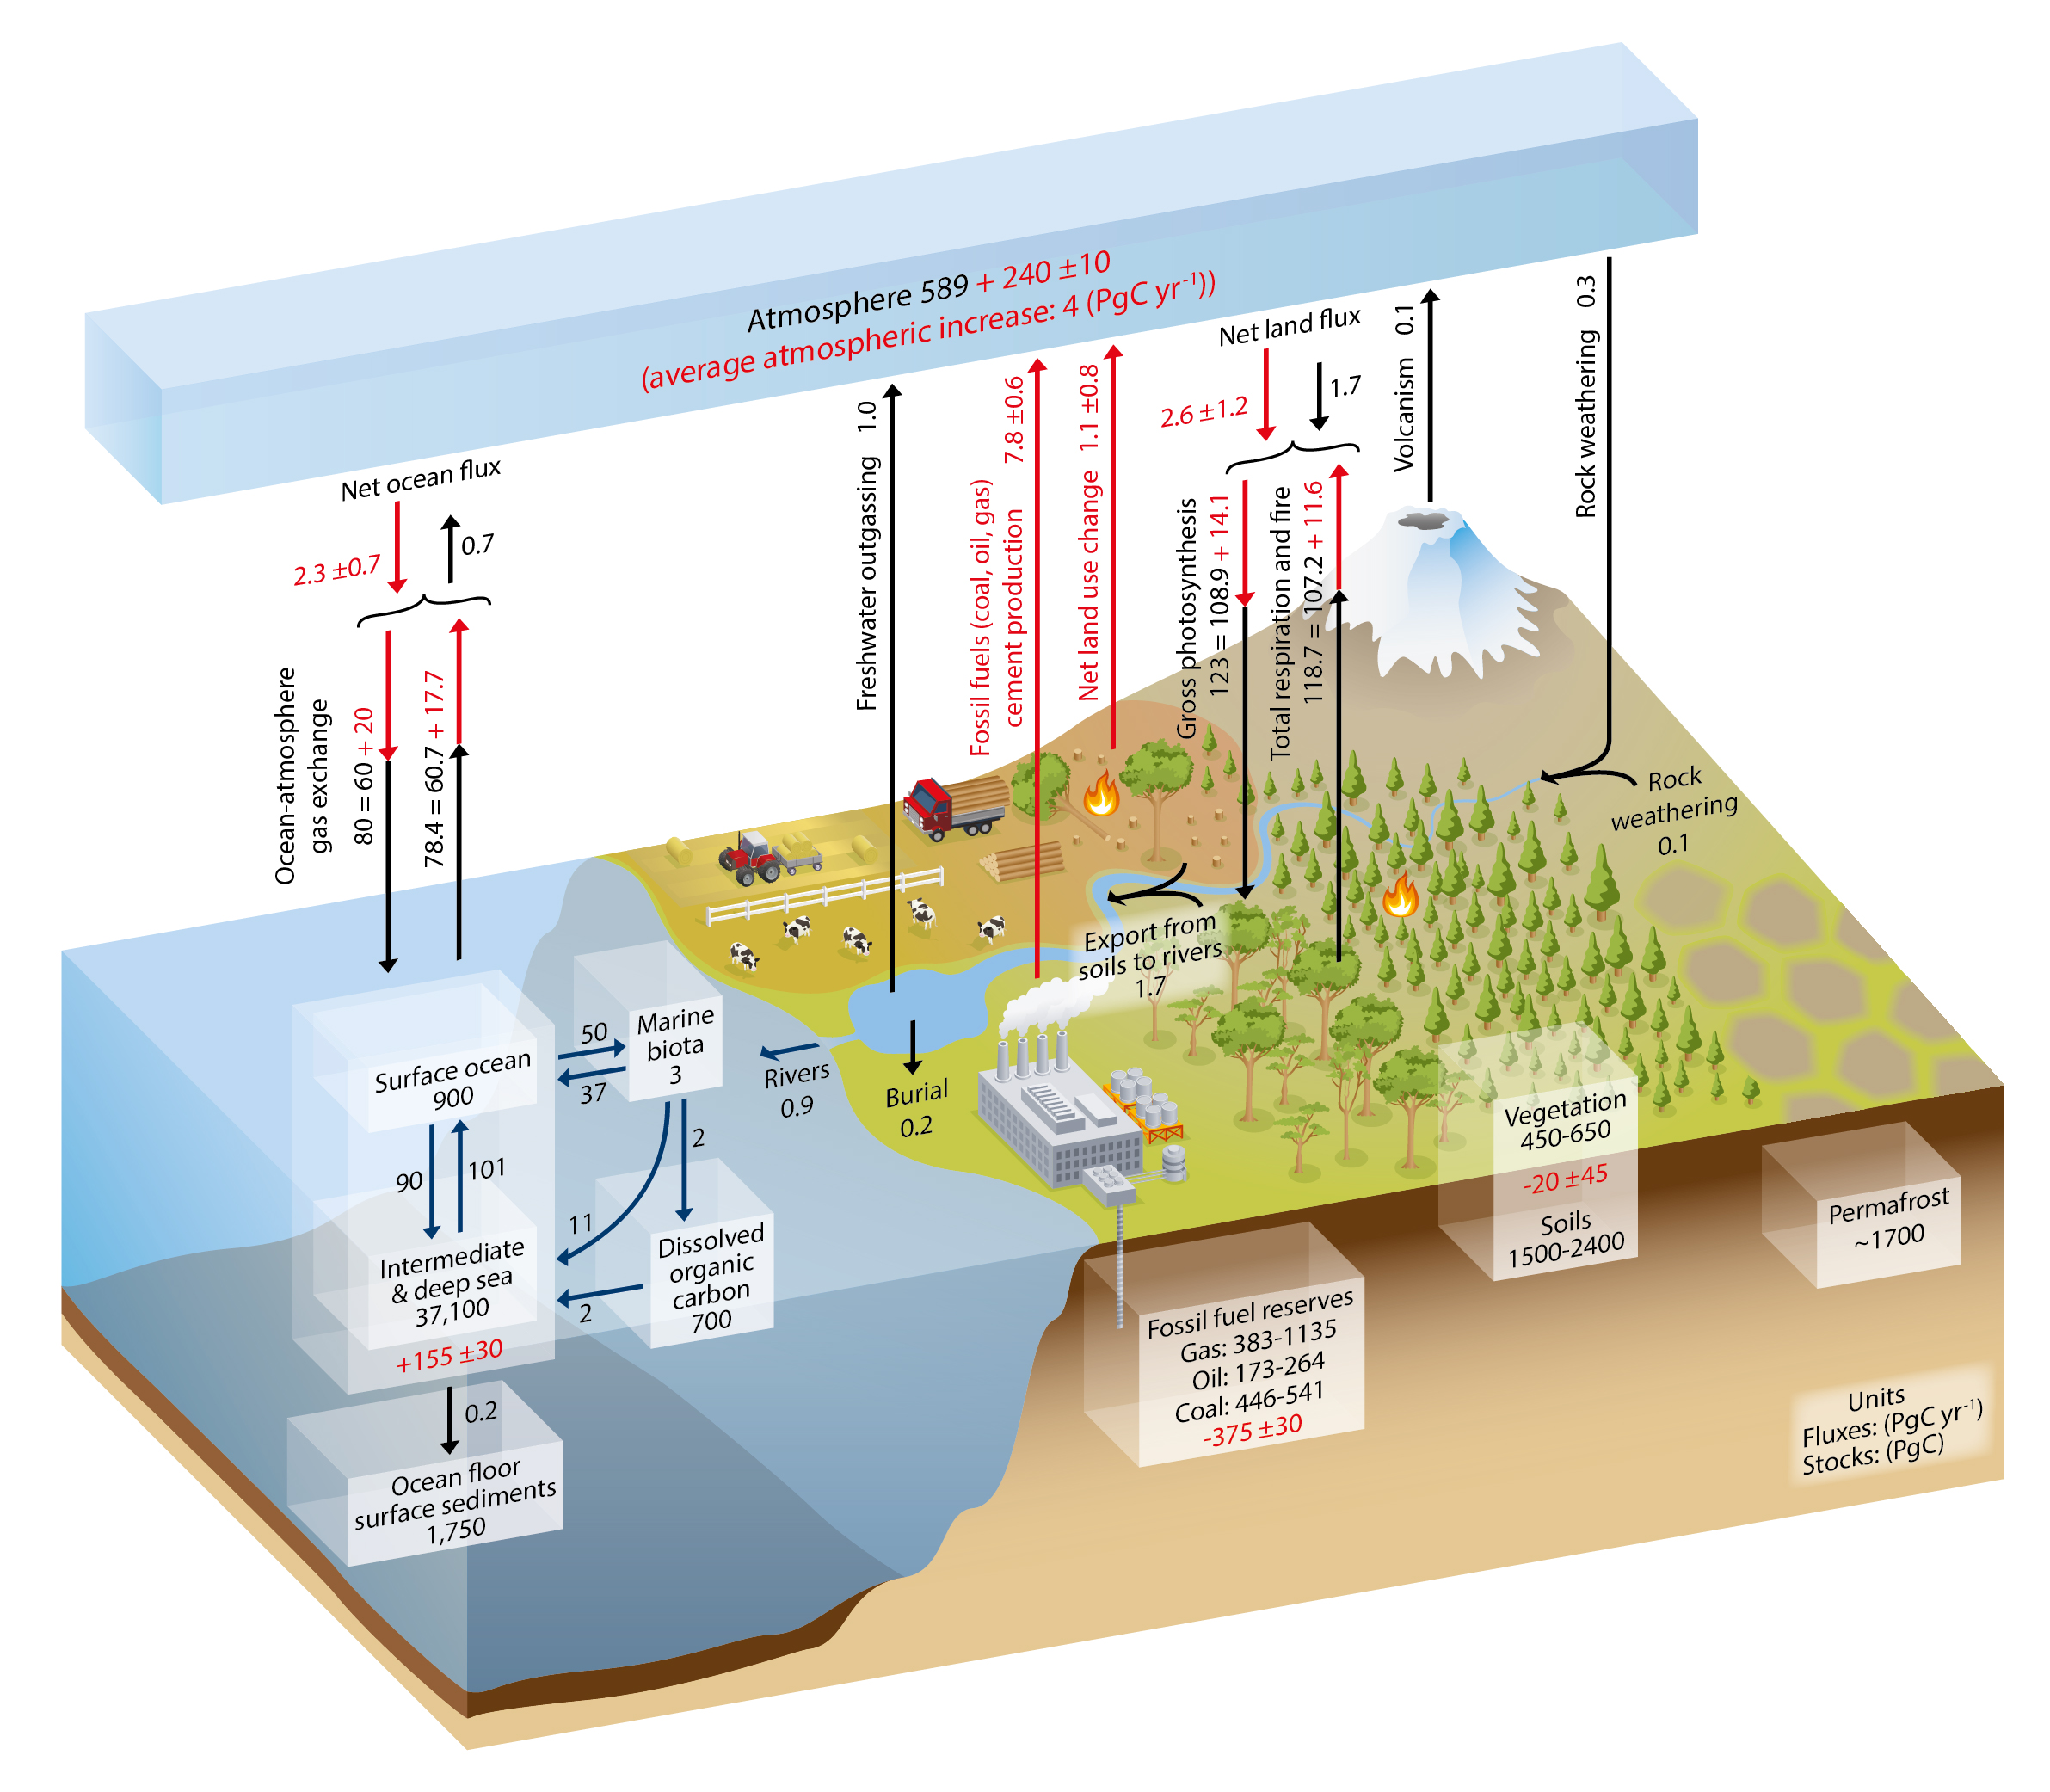
\includegraphics[width=0.9\textwidth]{chapter/chapter1/ipcc_fig6_1.jpg}
    \caption{Global carbon cycle simplified schematic \citep{ciais2014carbon}. Black numbers and arrows represent reservoir mass and exchange fluxes estimated for the time prior to the industrial era (\(\sim\)~1750). Red numbers and arrows represent annual fluxes averaged over the 2000-2009 time period. Red numbers in the reservoirs indicate the cumulative change of carbon over the industrial period (1750-2011).}
    \label{chap1:fig:ipcc_fig6.1}
\end{figure}

As atmospheric CO\(_{2}\) levels have risen, natural sinks of CO\(_{2}\) (fluxes out of the atmosphere) have intensified with both the land surface and oceans absorbing more CO\(_{2}\) from the atmosphere than in pre-industrial times. This can be see in figure~\ref{chap1:fig:ipcc_fig6.1}, with the the net ocean flux of CO\(_{2}\) to the atmosphere decreasing from an estimated +0.7~Pg~C~yr\(^{-1}\) to -2.3~Pg~C~yr\(^{-1}\), and the land surface flux of CO\(_{2}\) to the atmosphere decreasing from -1.7~Pg~C~yr\(^{-1}\) to -2.6~Pg~C~yr\(^{-1}\). More recent estimates from \citet{le2015global} indicate these sinks have further intensified with the ocean sink estimated to be 2.9 \(\pm 0.5\)~Pg~C~yr\(^{-1}\) and the land surface sink 4.1 \(\pm 0.9\)~Pg~C~yr\(^{-1}\) for the year 2014. The intensification of the land carbon sink is thought to be partly due to a combination of forest regrowth as well as rising CO\(_{2}\) and increased nitrogen deposition having a fertilisation effect \citep{ciais2014carbon}. It has also been shown that the land surface sink has been enhanced by an increase in diffuse photosynthetically active radiation as a result of increased cloud cover associated with increased anthropogenic emissions \citep{Mercadodiffuseradiation2009}. 

The partitioning of global carbon fluxes between emissions and sinks is important to better model the carbon cycle. However, current estimates are subject to high levels of uncertainty, which are reflected by the errors shown in Figure~\ref{chap1:fig:ipcc_fig6.1}. Current best estimates of global CO\(_{2}\) emissions and their partitioning between atmospheric growth rate and sinks are shown in Figure~\ref{chap1:fig:ipcc_fig6.8}. It is vitally important to understand the future response of sinks of CO\(_{2}\) (land surface and oceans) to climate change. If either the oceans or land surface were to stop absorbing the same percentage of CO\(_{2}\), we would see even more dramatic increases in atmospheric CO\(_{2}\) levels and thus a much greater rate of global warming. There is a high level of confidence that ocean carbon uptake will continue under all future emission scenarios \citep{ciais2014carbon}. There is much less confidence for the land surface and \citet{1748-9326-7-2-024002} have shown that global warming is particularly sensitive to land surface carbon cycle processes, highlighting the need to improve understanding of land surface carbon uptake. Some estimates show the land surface changing from a sink of CO\(_{2}\) to a source of CO\(_{2}\) under certain future emission scenarios \citep{sitch2008evaluation, cox2000, scholze2006climate}. In the latest IPCC report land surface carbon uptake is still considered the least understood process in the global carbon cycle \citep{ciais2014carbon}.

\begin{figure}[ht]
    \centering
    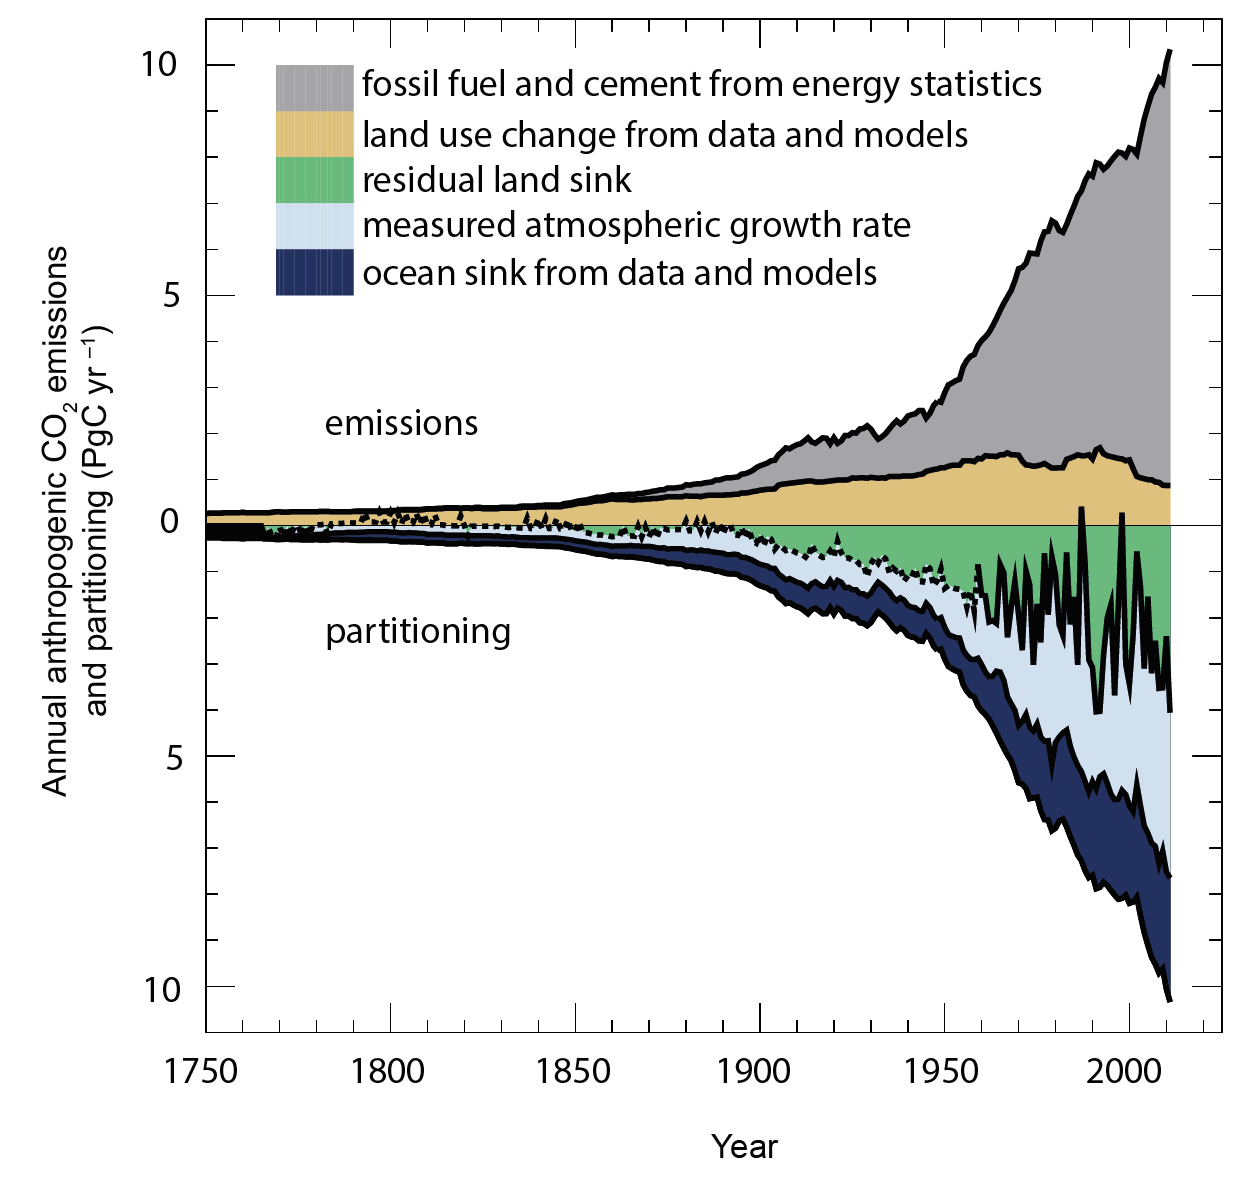
\includegraphics[width=0.9\textwidth]{chapter/chapter1/ipcc_fig6_8.jpg}
    \caption{Annual anthropogenic CO\(_{2}\) emissions and their partitioning among the atmosphere, land and ocean from 1750 to 2011  \citep{ciais2014carbon}.}
    \label{chap1:fig:ipcc_fig6.8}
\end{figure}

Currently land surface carbon uptake is estimated by taking the residual of all other calculated sources and sinks of carbon, so that
\begin{equation}
S_{LAND} = E_{FF} + E_{LUC} - (G_{ATM} + S_{OCEAN})
\end{equation}  
where \(S_{LAND}\) is the global residual land sink of CO\(_{2}\), \(E_{FF}\) is the CO\(_{2}\) emissions from fossil fuels, \(E_{LUC}\) is the CO\(_{2}\) emissions from land use change (mainly deforestation), \(G_{ATM}\) is the atmospheric CO\(_{2}\) growth rate and \(S_{OCEAN}\) is the mean ocean CO\(_{2}\) sink \citep{le2015global}. Figure~\ref{chap1:fig:ipcc_fig6.8} shows the growth in the estimated residual land sink as emissions increase. The high variability shown in this sink is largely due to the fact that it contains the residual errors of the four other terms. However, the land sink also displays some variability due to its sensitivity to year to year variations in precipitation, surface temperature, radiation and volcanic eruptions. Figure~\ref{chap1:fig:ipcc_fig6.8} shows that in 1986 and 1997 the land sink drops to zero, both of these years were among the strongest El Ni\~no's in recent history. In 1997 tropical droughts, often associated with El Ni\~no, were particularly severe leading to wildfires that released vast amounts of stored carbon \citep{schimel2013climate}.

%{\color{red} Include ecosystem flux description and figure here}
Terrestrial ecosystems are made up of autotrophs (organisms capable of photosynthesis) and heterotrophs (organisms that feed on organic carbon). The Gross Primary Productivity (GPP) of an ecosystem is the total amount of carbon removed from the atmosphere by photosynthesis. The Total Ecosystem Respiration (TER) is made up of autotrophic respiration (e.g. from plants) and heterotrophic respiration (e.g. from soil and litter organisms). The total carbon uptake or Net Ecosystem Exchange (NEE) of CO\(_2\) is then equal to -GPP+RT. A representation of these fluxes for a forest ecosystem are shown in Figure~\ref{chap1:fig:eco_fluxes}. 

\begin{figure}[ht]
    \centering
    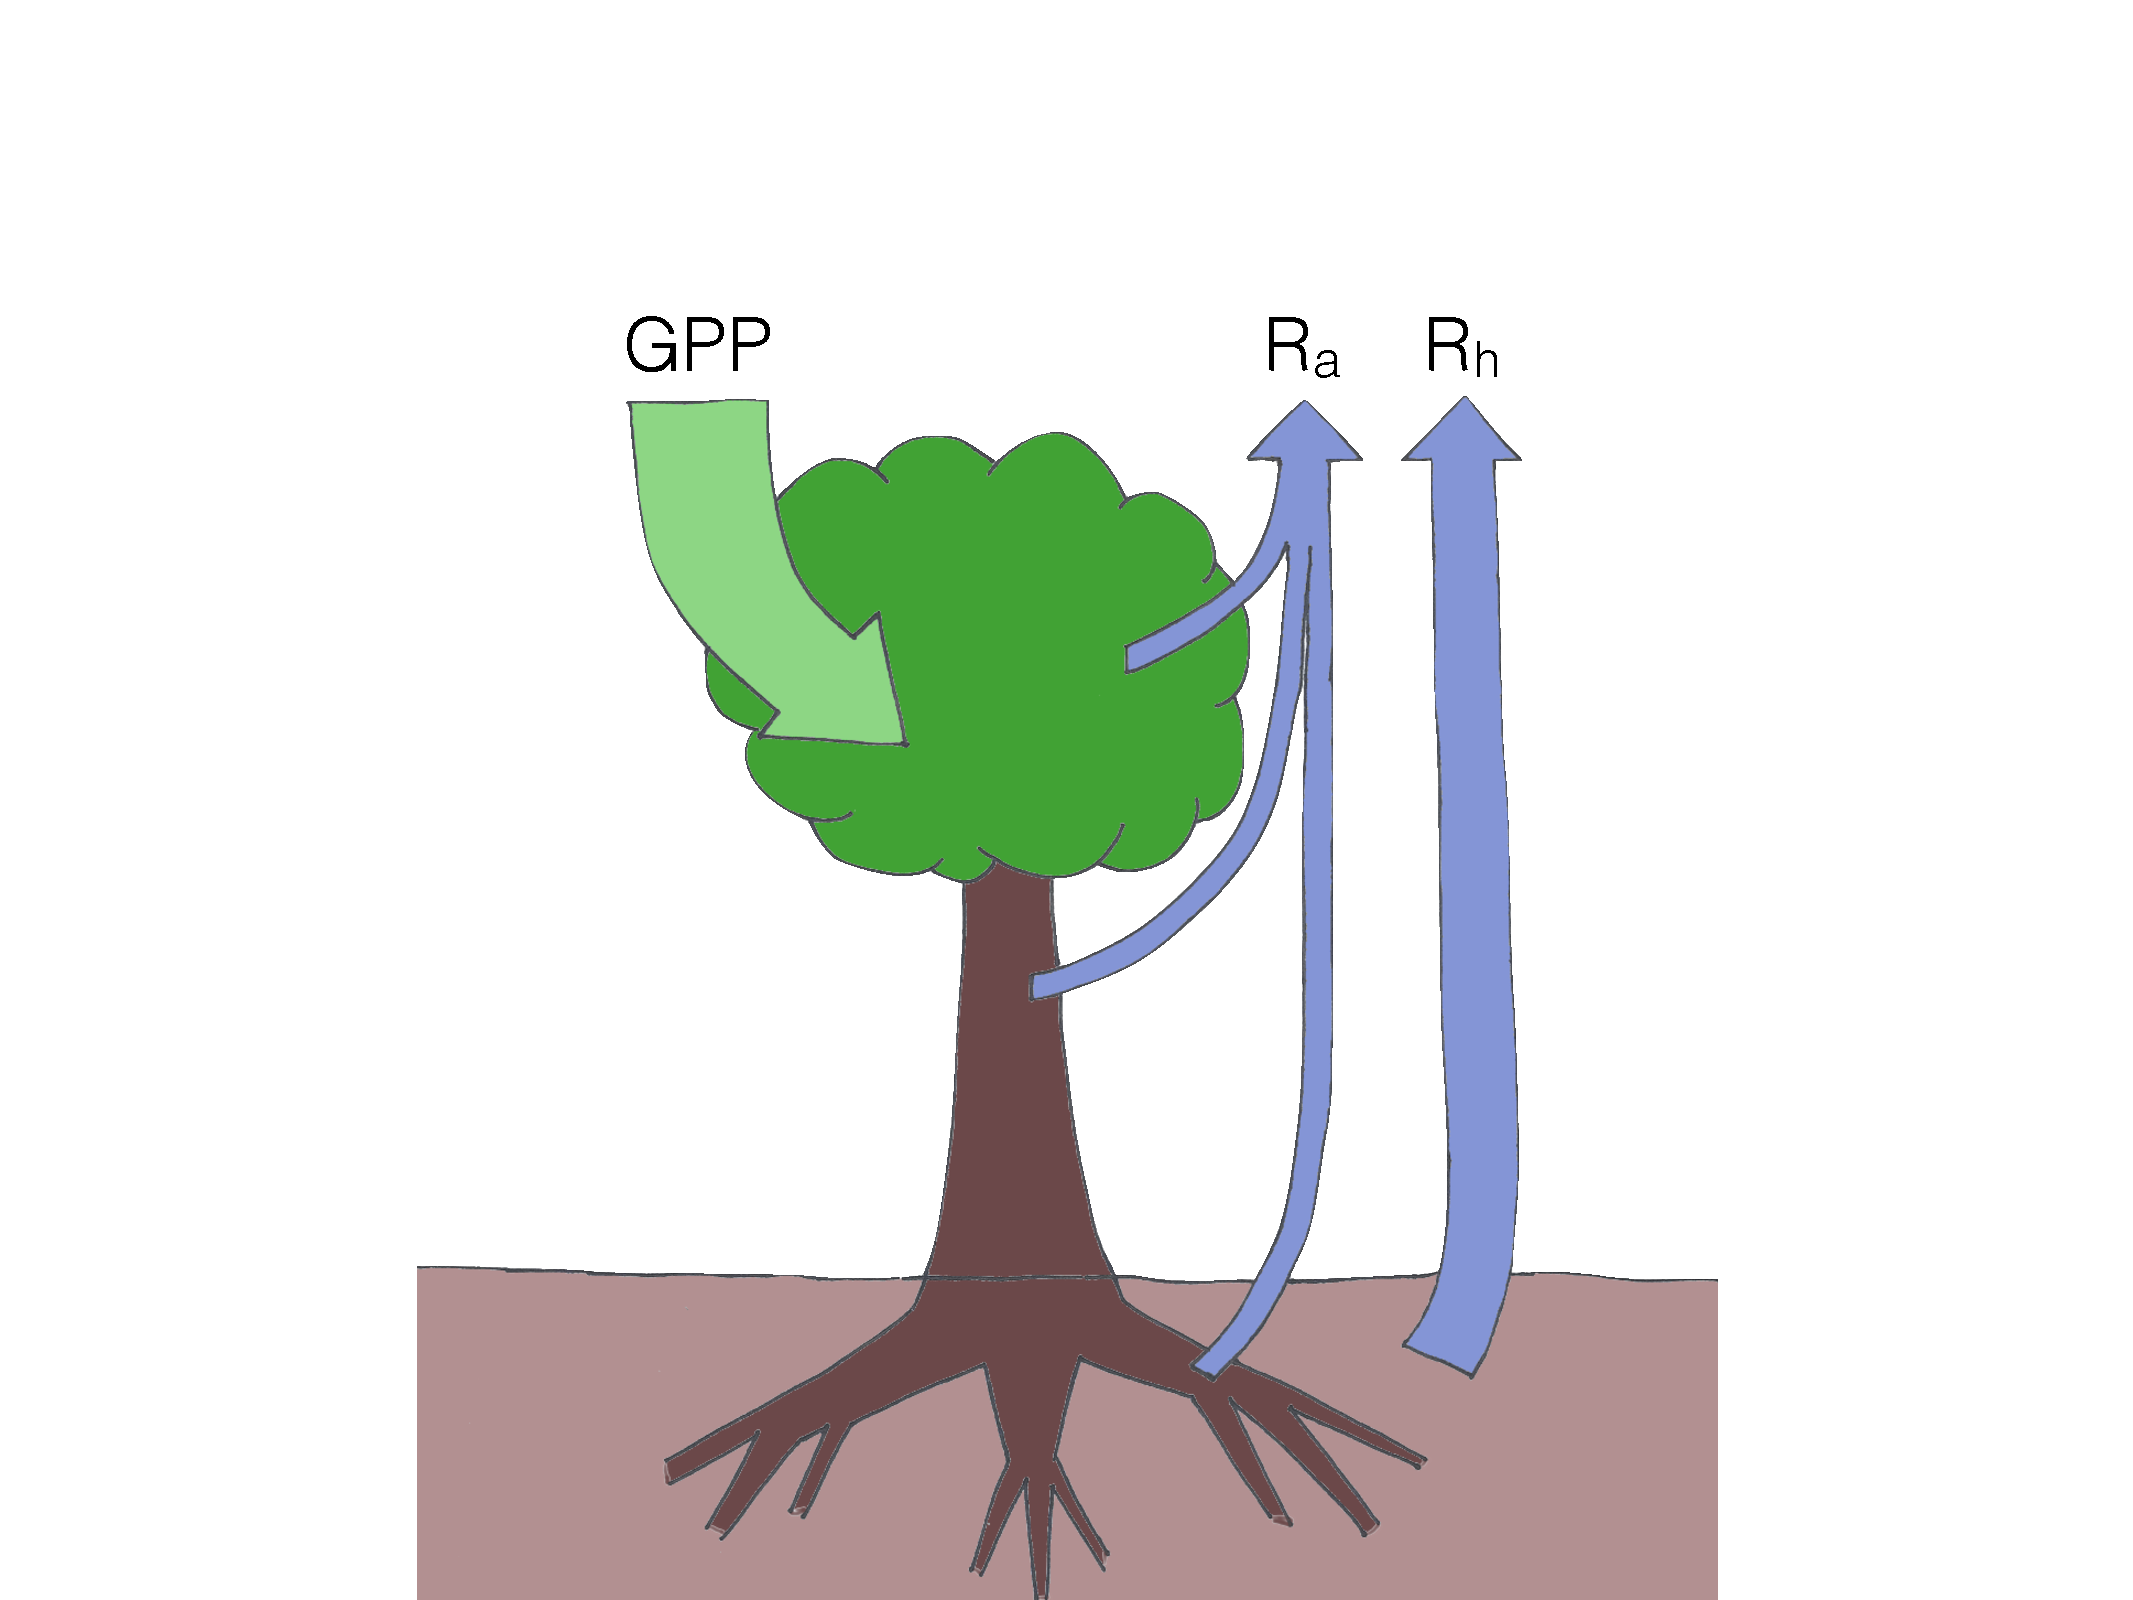
\includegraphics[width=0.5\textwidth]{chapter/chapter1/flux.pdf}
    \caption{Fluxes of carbon through a forest ecosystem. Gross Primary Productivity (GPP) represents total photosynthesis, R\(_{\text{a}}\) is autotrophic respiration from foliage, wood and roots, R\(_{\text{h}}\) is heterotrophic respiration from soil and litter. Total ecosystem respiration of carbon to the atmosphere (RT) is equal to R\(_{\text{a}}\) + R\(_{\text{h}}\). The Net Ecosystem Exchange (NEE) of CO\(_{2}\) is equal to -GPP + RT.}
    \label{chap1:fig:eco_fluxes}
\end{figure}

Disturbance of terrestrial ecosystems from fire, felling and insect outbreak can have significant impacts on carbon dynamics. Land use change is the second largest anthropogenic source of CO\(_{2}\). However, It is not well understood how much CO\(_{2}\) is removed from the atmosphere by regrowth of previously disturbed ecosystems (either by felling or fire), although it is thought that regrowth of forests in partcular could be stronger carbon sinks than their predecessors, due to more rapid biomass accumulation under succession \citep{pan2011large}. Better understanding the response of the land surface to disturbance will help constrain future carbon budgets. 

%Good paper to highlight the fact that the percentage of CO\(_{2}\) absorbed by the land surface has remained approximately constant with rising atmospheric CO\(_{2}\) levels??? Maybe just use IPCC fig 6.8?

%In figure 6.1 and 6.8: Partitioning of fluxes important and hard (shown by error on estimates in fig 6.1). Land surface carbon uptake least understood mechanism in the global carbon cycle, ref IPCC. Will uptake remain the same under climate change.

%Human emissions of CO\(_{2}\) have perturbed the global C cycle and caused a large continual increase in atmospheric CO\(_{2}\) levels.

%Look at papers recommended on Flux Course, some good ones to reference???

%IPCC figure 6.1 and 6.8: Partitioning of fluxes important and hard (shown by error on estimates in fig 6.1). Land surface carbon uptake least understood mechanism in the global carbon cycle, ref IPCC. Will uptake remain the same under climate change.

%\citet{1748-9326-7-2-024002} Have shown that global warming is highly sensitive to land carbon cycle processes and highlighted the need to improve understanding of land surface carbon uptake and its response to climate change. 

\subsection{Observations of terrestrial carbon balance}

There are an increasing number of available observations relevant to understanding the carbon balance of forests and the terrestrial biosphere. These observations include a range of variables, perhaps two of the most common are the Net Ecosystem Exchange (NEE) of CO\(_{2}\) and Leaf Area Index (LAI), which is the area of leaves per unit area ground. These variables can be directly measured at site level and can also be estimated from satellite remote sensing. Both NEE and LAI are important variables for understanding the carbon balance of ecosystems, with NEE giving us a direct estimate of the carbon uptake of an ecosystem and LAI being a main driver for the amount of GPP an ecosystem can perform.

%para on flux network and site level data:
At site level, flux towers measuring ecosystem-atmosphere fluxes of CO\(_{2}\), water and energy using the micrometeorological technique of eddy covariance provide one of the most valuable sources of information. Direct observations of ecosystem CO\(_{2}\) uptake are made at a fine temporal resolution, with observations every half-hour. A global flux network (FLUXNET), was established in 1997 \citep{baldocchi2001fluxnet}, to consolidate the information from a growing number of flux tower sites. Currently there are 517 active FLUXNET sites which are shown in Figure~\ref{chap1:fig:fluxnet_2015}, as can be seen these sites are not uniformly distributed so it is not possible to use FLUXNET sites alone to produce global estimates of terrestrial CO\(_{2}\) balance. However, these sites do provide an invaluable resource for model and satellite calibration. In turn this can be used to produce estimates on a global scale. At many flux tower sites and forest stands other diverse observations relevant to terrestrial carbon budgets are also being made. These include observations of soil and litter respiration, woody biomass and LAI. However, because they are labour intensive these observations are made much less frequently.     

\begin{figure}[ht]
\centering
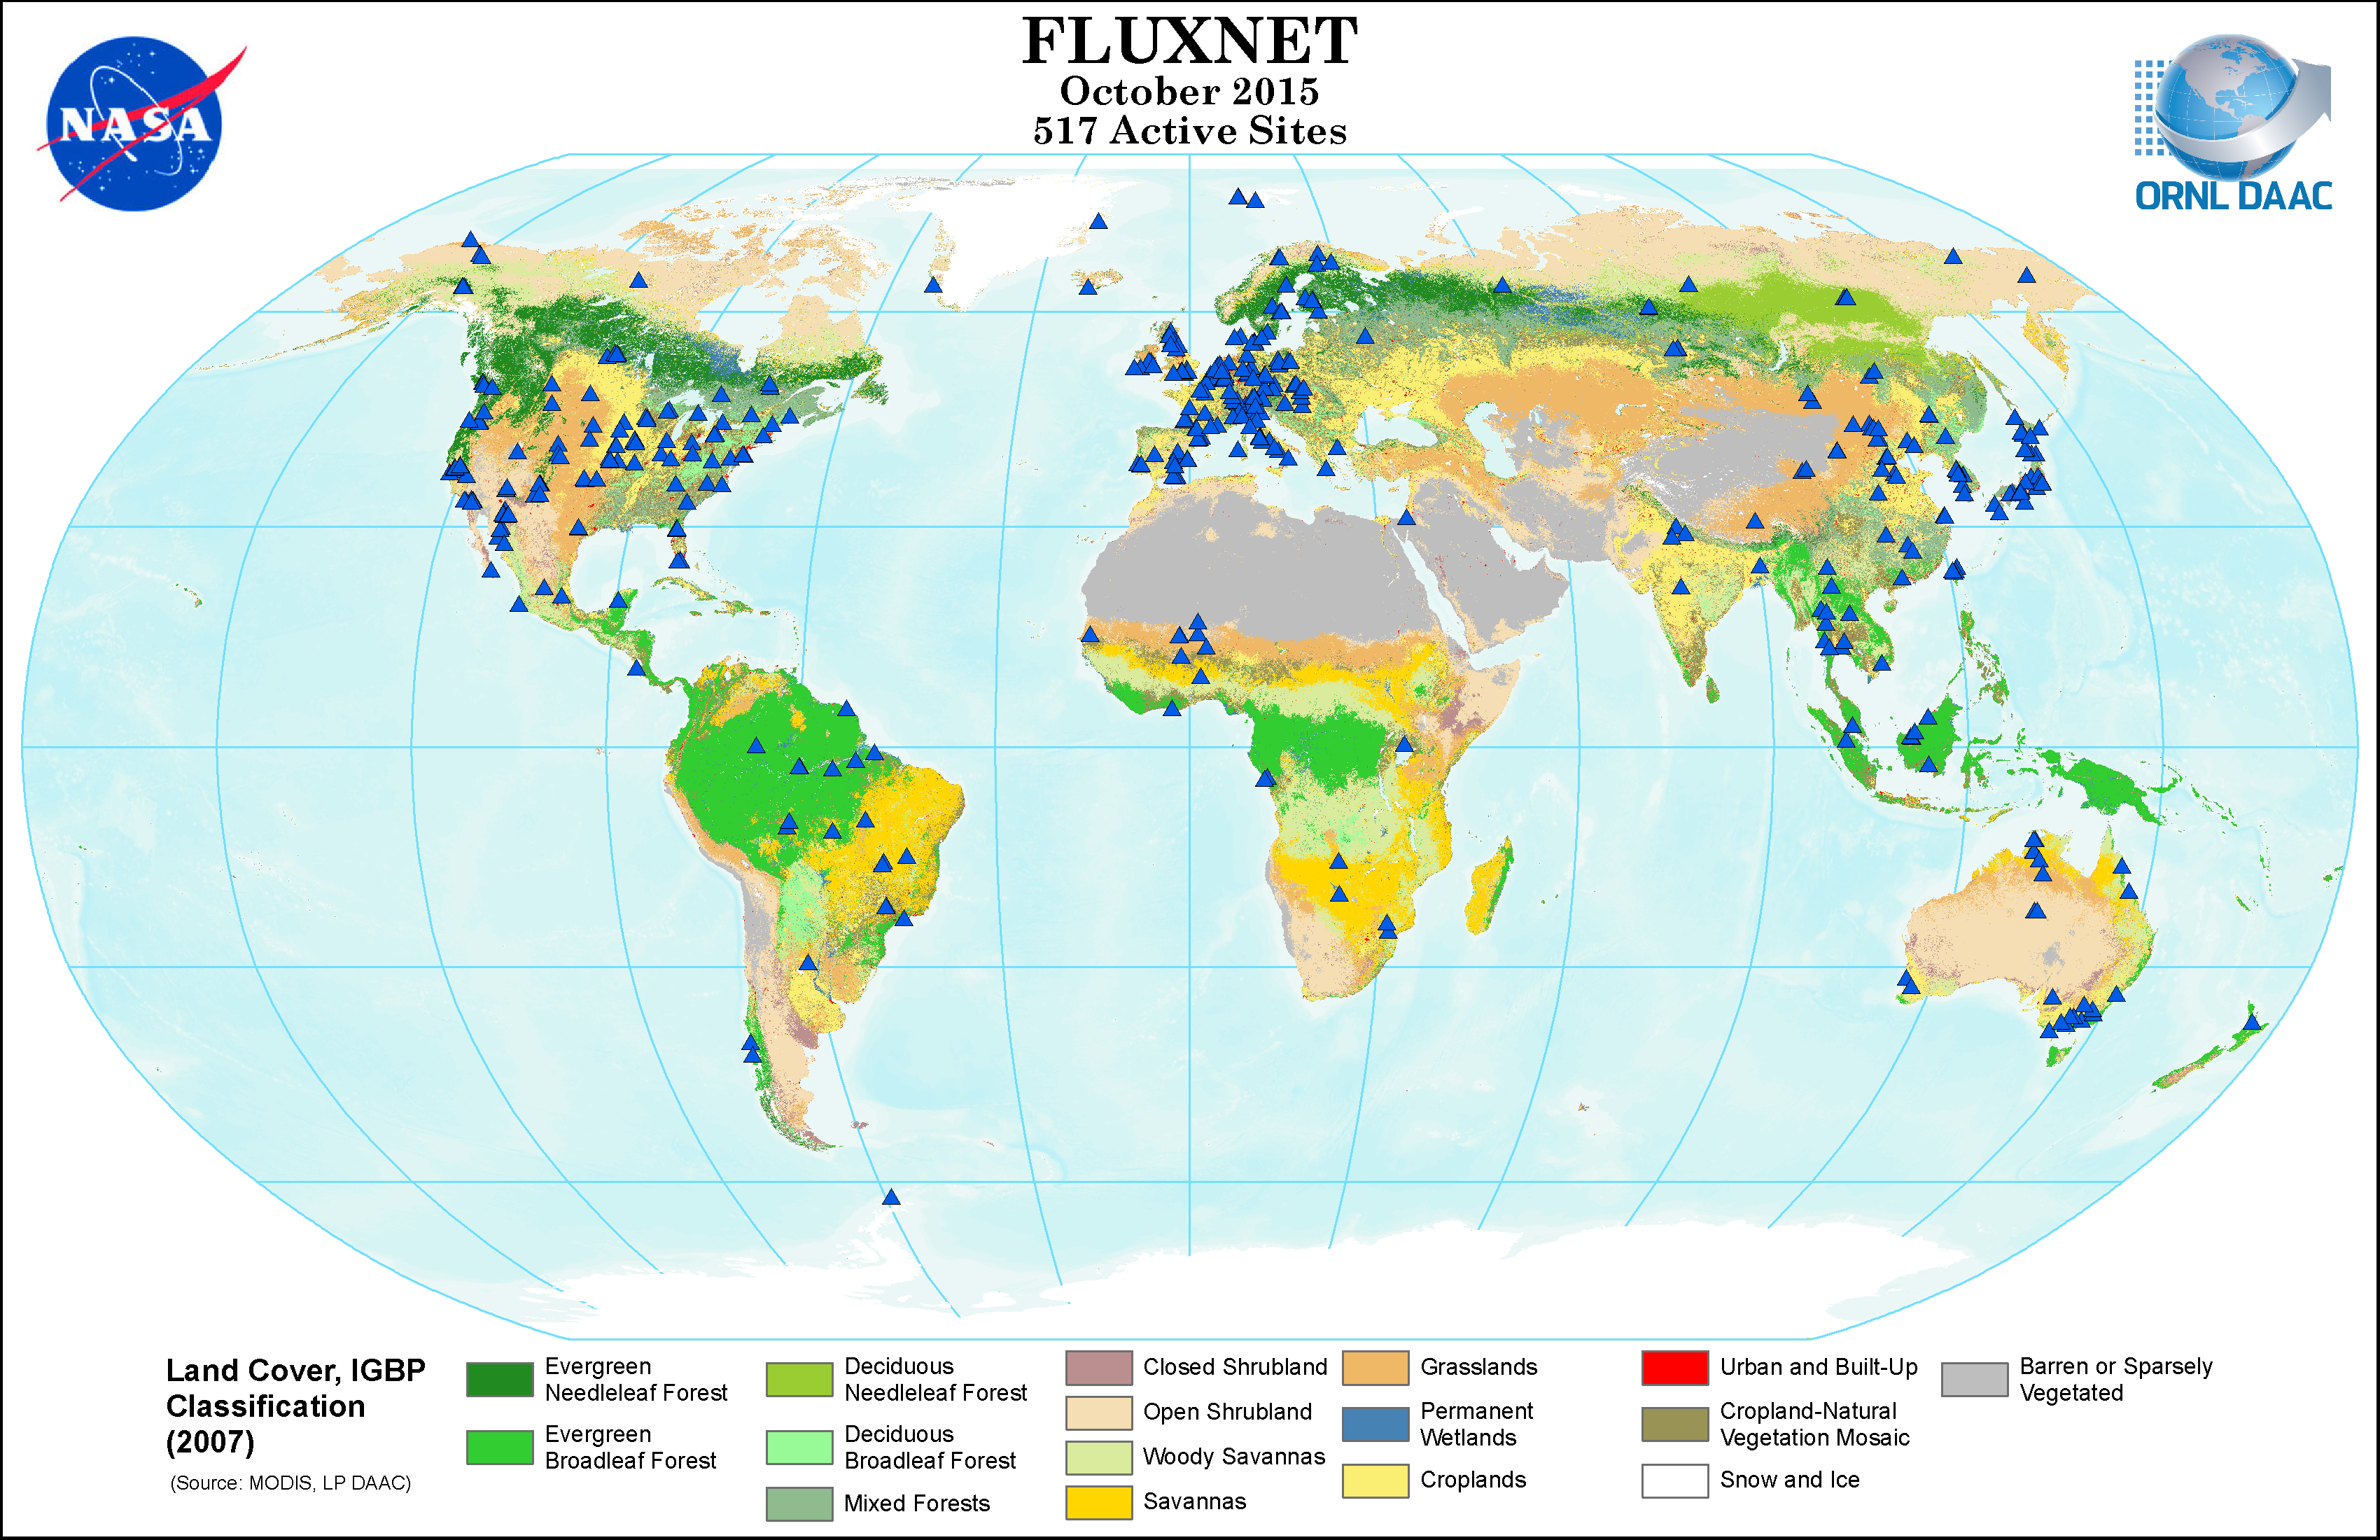
\includegraphics[width=0.9\textwidth]{chapter/chapter1/FluxNetworkMODIS_IGBP_10-2015.png}
\caption{FLUXNET sites and land cover (MODIS IGBP classification) \citep{fluxnetsite2013}.}
\label{chap1:fig:fluxnet_2015}
\end{figure}

%para on satellite data
The Moderate Resolution Imaging Spectroradiometer (MODIS) on the TERRA and AQUA satellites produces global estimates of LAI and Gross Primary Productivity (GPP) for terrestrial ecosystems \citep{running2004continuous}. However, MODIS actually measures reflected sunlight, this is then converted to vegetation indices, such as the Normalised Difference Vegetation Index (NDVI). These indices are correlated with the fraction of absorbed visible sunlight to estimate LAI or used in simple algorithms to estimate GPP \citep{yuan2007deriving}. It is therefore important to understand the limitations when interpreting satellite products as they do not represent direct observations. For LAI it has been shown that remotely sensed estimates saturate when measuring ecosystems with a LAI above 3 \citep{myneni2002global}. Terrestrial fluxes of carbon estimated from satellite measurements are subject to large errors in representativity, as satellites view a scene almost instantaneously and then derive daily mean fluxes \citep{baldocchi2008turner}. 
%Baldocchi paper: Many observations of forest carbon flux made worldwide.

\subsection{The role of models}

Observations can only tell us about the current and past state of a system. In order to produce future predictions and better understand current terrestrial carbon dynamics we must use mathematical models. Figure~\ref{chap1:fig:ipcc_fig6.16} show a comparison of the residual land sink (described in section~\ref{chap1:sec:global_c_cycle}) with the global terrestrial CO\(_{2}\) sink estimated from different process based global carbon cycle models. We see that although there is a high variability between modelled estimates there is good agreement between the multi-model mean and the residual land sink. 

\begin{figure}[ht]
    \centering
    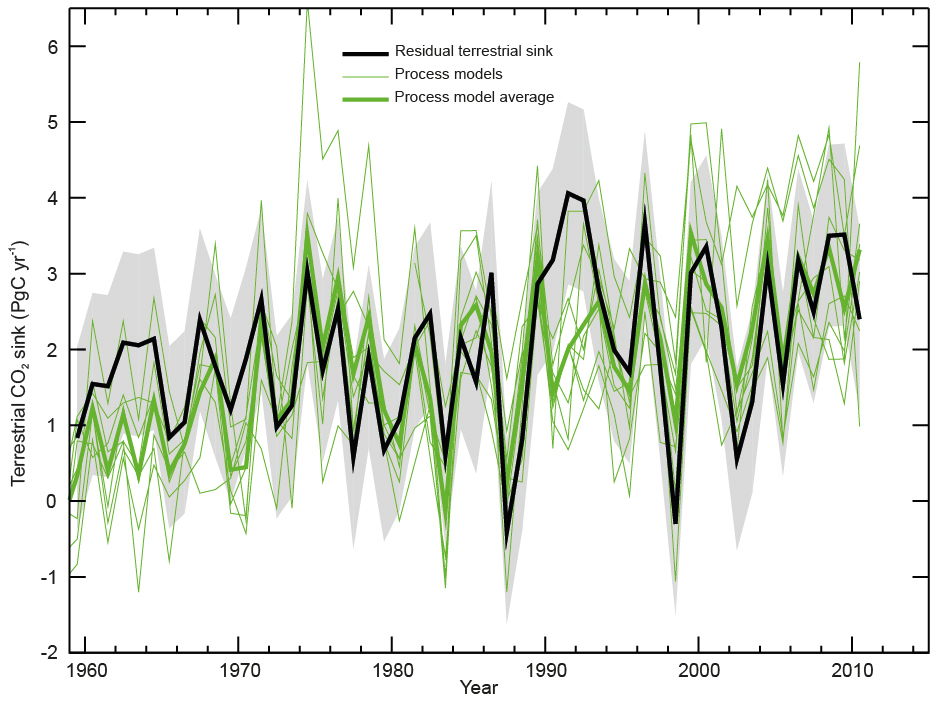
\includegraphics[width=0.9\textwidth]{chapter/chapter1/ipcc_fig6_16.jpg}
    \caption{Comparison of the residual land sink (black line) with the global terrestrial CO\(_{2}\) sink estimated from different process based global carbon cycle models \citep{ciais2014carbon}. Grey shading represents uncertainty in residual land sink.}
    \label{chap1:fig:ipcc_fig6.16}
\end{figure}

Representative Concentration Pathways (RCPs) of CO\(_{2}\) concentrations and emissions have been developed \citep{moss2010next} to drive climate models to produce future predictions. Under these pathways land surface carbon uptake is highly uncertain with little agreement between different process based models. Some predict the land surface to become a source of CO\(_{2}\) and others predict a further intensification of the residual land sink \citep{jones2013twenty}. This large uncertainty for land surface models is partly due to poor model parameterisations and missing processes within models. One of the main processes many current global models do not account for is the effect of disturbance on terrestrial ecosystem carbon dynamics.

It has been shown that many terrestrial carbon cycle models simulating the seasonal cycle of land-atmosphere CO\(_{2}\) exchange perform poorly when compared to FLUXNET sites in North America \citep{schwalm2010model}. Here a difference between observations and model predictions of 10 times the observational uncertainty was found, highlighting the need for continued model development. In order to improve global models of terrestrial carbon balance it is important to use site-level-research to hone the processes and parameterisations of the models where we have diverse sets of direct observations with which to judge modified-model performance. 
%IPCC figure 6.16 and section 6.3.2.6.6: Contribution of models to understanding the terrestrial carbon cycle. Reference every DALEC paper.


\subsection{Data assimilation}

%{\color{red} Observations are sparse, current model predictions are poor, data assimilation provides a way to combine both sources of information to improve current estimates.}

As discussed above, the level of uncertainty in terrestrial carbon balance predictions arise from significant gaps in the direct observations available and from a lack of clarity and authoritative parameterisation of the constituent processes in current models. The technique of data assimilation provides a method for combining and comparing the output of predictive models with incomplete observations to find the best estimate for the state and parameters of a system. Data assimilation has had many successful applications. Perhaps the most important application has been in numerical weather prediction where data assimilation has contributed to forecast accuracy being increased at longer lead times, with the result that the four day forecast in 2014 now has the same level of accuracy as the one day forecast in 1979 \citep{bauer2015quiet}. Obviously, this improved forecasting is not solely due to data assimilation but also increased quality and resolution of observations along with improvements in model structure, however the introduction and evolution of data assimilation has been a key part of the improvement \citep{dee2011era}.

More recently data assimilation has been used to improve our knowledge of ecological systems. For the carbon balance of forests it has been used to combine many different observations with functional ecology models \citep{zobitz2011primer, fox2009reflex, richardson2010estimating, Quaife2008, Zobitz2014, Niu2014}. Global land surface models have also been implemented with data assimilation, mainly using data from satellite and atmospheric $\text{CO}_{2}$ observations \citep{Kaminski2013, scholze2007propagating}. In a few cases site level data has also been assimilated \citep{Verbeeck2011, Bacour2015}. In comparison with numerical weather prediction, the use of data assimilation in these areas is relatively new and underdeveloped. The further application of data assimilation to models of ecosystem carbon balance will help to improve model parameterisations and future predictions. The development of improved data assimilation techniques will also help to  identify missing model processes and changes in model parameters and behaviour over time. In particular, understanding the change in model parameters over time will be of use in improving models predictions of the effect of disturbance in terrestrial ecosystems.
  
%Role of DA in NWP improving forecast skill. 

\section{Thesis aims}

The primary aim of this thesis is the development of data assimilation techniques for the terrestrial carbon cycle, in order to aid progress in this field of research. We focus on implementing novel data assimilation methods with a simple model of ecosystem carbon balance in order to address three key areas:

\begin{enumerate}
\item \textit{Investigating the information content in distinct carbon balance observations for data assimilation}

It is important to understand which observations provide most information to data assimilation schemes. We investigate the different relative levels of information for observations relevant to ecosystem carbon balance through novel applications of information content metrics.

\item \textit{Improving the representation of prior and observational errors in carbon cycle data assimilation}

Currently the specification of both prior and observational errors for the carbon cycle have been simplistic. We seek to improve this representation by investigating the role of correlations between errors for both prior estimates and observations. We judge the effect of including these error correlations on data assimilation results.
  
\item \textit{Using data assimilation to understand the effect of disturbance on forest carbon dynamics}

The effect of disturbance (e.g. fire, felling, insect outbreak) on ecosystem carbon dynamics is one of the least understood components of the global carbon cycle. We investigate the effect of selective felling on forest carbon uptake using novel data assimilation techniques.
\end{enumerate}

\section{Thesis outline}

From this point onwards the thesis is structured as follows:

\begin{itemize}
\item \textbf{Chapter~\ref{chap:litrev}} introduces the concept of data assimilation and relevant methods. In particular applications of data assimilation to the terrestrial carbon cycle are discussed. We highlight some of the current issues faced and areas for future development.  

\item \textbf{Chapter~\ref{chap:data}} provides an explanation of the Data Assimilation Linked Ecosystem Carbon (DALEC1 and DALEC2) models used throughout the thesis. The fieldwork campaign conducted during this PhD project is outlined along with additional flux tower data from the Alice Holt research site (Hampshire, UK).

\item \textbf{Chapter~\ref{chap:info_con}} explores the first aim of the thesis. The DALEC1 and DALEC2 model are are used in a set of information content experiments, with novel applications of information content metrics, in order to better understand the relative levels of information from different observations and how information content might vary in time and with different characterisations of errors.

\item \textbf{Chapter~\ref{chap:error_corrs}} introduces a fully tested data assimilation scheme with the DALEC2 model and uses this to address the second aim of the thesis. The role of prior and observation error correlations are investigated in a set of data assimilation experiments to understand their contribution to improving a model forecast of forest carbon uptake.

\item \textbf{Chapter~\ref{chap:disturbance}} uses the techniques developed in chapter~\ref{chap:error_corrs} along with supplementary observations from the fieldwork campaign outlined in chapter~\ref{chap:data} to address the third aim of the thesis.

\item \textbf{Chapter~\ref{chap:conclusion}} presents the results of the thesis as a whole and discusses opportunities for future work.    

\end{itemize}

